% fig17-followup-provider-splits.tex
% Paper-freeze lesion outcomes for the closeout cohort
\documentclass[tikz,border=18pt]{standalone}
% common-styles.tex
% Shared TikZ styles for wonton-proof paper figures

\usepackage{silence}
\WarningFilter{latex}{Missing character} 
\tracinglostchars=0 % Suppress engine-level "Missing character" warnings

\usepackage{fontspec}
\usepackage{unicode-math}

% Use filenames for reliability with Tectonic
\setmainfont{LibertinusSerif-Regular.otf}[
    BoldFont=LibertinusSerif-Bold.otf,
    ItalicFont=LibertinusSerif-Italic.otf,
    BoldItalicFont=LibertinusSerif-BoldItalic.otf
]
\setsansfont{LibertinusSans-Regular.otf}[
    BoldFont=LibertinusSans-Bold.otf,
    ItalicFont=LibertinusSans-Italic.otf
]
\setmonofont{LibertinusMono-Regular.otf}

% Try a more standard math font if LibertinusMath is causing nullfont issues
\setmathfont{LibertinusMath-Regular.otf}
% \setmathfont{latinmodern-math.otf}[range=digits] 

\usepackage{amsmath}
\usepackage{tikz}
\usepackage{forest}

\usetikzlibrary{
    arrows.meta,
    calc,
    decorations.pathreplacing,
    fit,
    positioning,
    shapes.geometric,
    shapes.misc,
    backgrounds,
    shadows.blur,
    fadings
}

% Color palette (muted, print-friendly)
\definecolor{ink}{RGB}{45,45,52}
\definecolor{muted}{RGB}{115,115,125}
\definecolor{highlight}{RGB}{198,120,44}
\definecolor{accentblue}{RGB}{86,130,178}
\definecolor{accentgreen}{RGB}{84,156,132}
\definecolor{blocked}{RGB}{140,75,75}
\definecolor{goalnode}{RGB}{255,255,255}
\definecolor{terminal}{RGB}{238,239,244}
\definecolor{deadnode}{RGB}{248,245,245}
\definecolor{flowbox}{RGB}{250,250,252}
\definecolor{basin1}{RGB}{224,234,248}
\definecolor{basin2}{RGB}{246,232,221}
\definecolor{basin3}{RGB}{228,242,234}
\definecolor{heatbase}{RGB}{86,130,178}

\tikzset{
    line cap=round,
    line join=round,
    pop/.style={
        blur shadow={shadow blur steps=5, shadow blur extra rounding=1.3pt}
    },
    base node/.style={
        rounded rectangle,
        draw=ink,
        line width=0.6pt,
        fill=goalnode,
        text=ink,
        minimum width=2.2cm,
        minimum height=0.7cm,
        align=center,
        pop
    },
    goal/.style={base node, fill=goalnode},
    terminal/.style={base node, fill=terminal, line width=0.9pt},
    dead/.style={base node, fill=deadnode, dashed},
    flowbox/.style={
        rectangle,
        draw=muted,
        rounded corners=3pt,
        fill=flowbox,
        minimum width=1.8cm,
        minimum height=0.6cm,
        align=center,
        font=\normalfont\small,
        text=ink,
        pop
    },
    decision/.style={
        diamond,
        draw=muted,
        fill=flowbox,
        aspect=2.4,
        font=\normalfont\small,
        inner sep=1pt,
        text=ink
    },
    protocolbox/.style={
        rectangle,
        draw=muted,
        rounded corners=4pt,
        fill=flowbox,
        minimum width=2cm,
        minimum height=0.8cm,
        font=\normalfont\small,
        align=center,
        text=ink
    },
    tactic/.style={
        ->,
        >=Stealth,
        draw=muted,
        line width=0.75pt
    },
    tacticlight/.style={
        ->,
        >=Stealth,
        draw=muted!45,
        dashed,
        line width=0.6pt
    },
    backprop/.style={
        ->,
        >=Stealth,
        draw=muted!70,
        dashed,
        line width=0.6pt
    },
    selected/.style={
        tactic,
        draw=highlight,
        line width=1.4pt
    },
    divergetactic/.style={
        tactic,
        draw=highlight,
        line width=1.4pt
    },
    divergenode/.style={
        base node,
        draw=highlight,
        line width=1.0pt
    },
    divergeblock/.style={
        blockedtactic,
        line width=1.2pt
    },
    blockedtactic/.style={
        tactic,
        draw=blocked,
        densely dashed
    },
    flowarrow/.style={
        ->,
        >=Stealth,
        draw=muted,
        line width=0.75pt
    },
    crosslink/.style={
        -,
        draw=muted!70,
        dotted,
        line width=0.6pt
    },
    annot/.style={
        font=\normalfont\footnotesize,
        text=muted
    },
    visit/.style={
        annot,
        font=\normalfont\scriptsize
    },
    annotbg/.style={
        annot,
        fill=white,
        inner sep=1.5pt
    },
    tacticlabel/.style={
        annot,
        font=\ttfamily\footnotesize,
        text=muted
    },
    formula/.style={
        font=\normalfont\footnotesize,
        draw=muted,
        rounded corners=2pt,
        fill=white,
        inner sep=3pt
    },
    paneltitle/.style={
        font=\normalfont\bfseries,
        text=ink
    },
    trajectory/.style={
        ->,
        draw=muted!70,
        line width=0.6pt
    }
}


\begin{document}
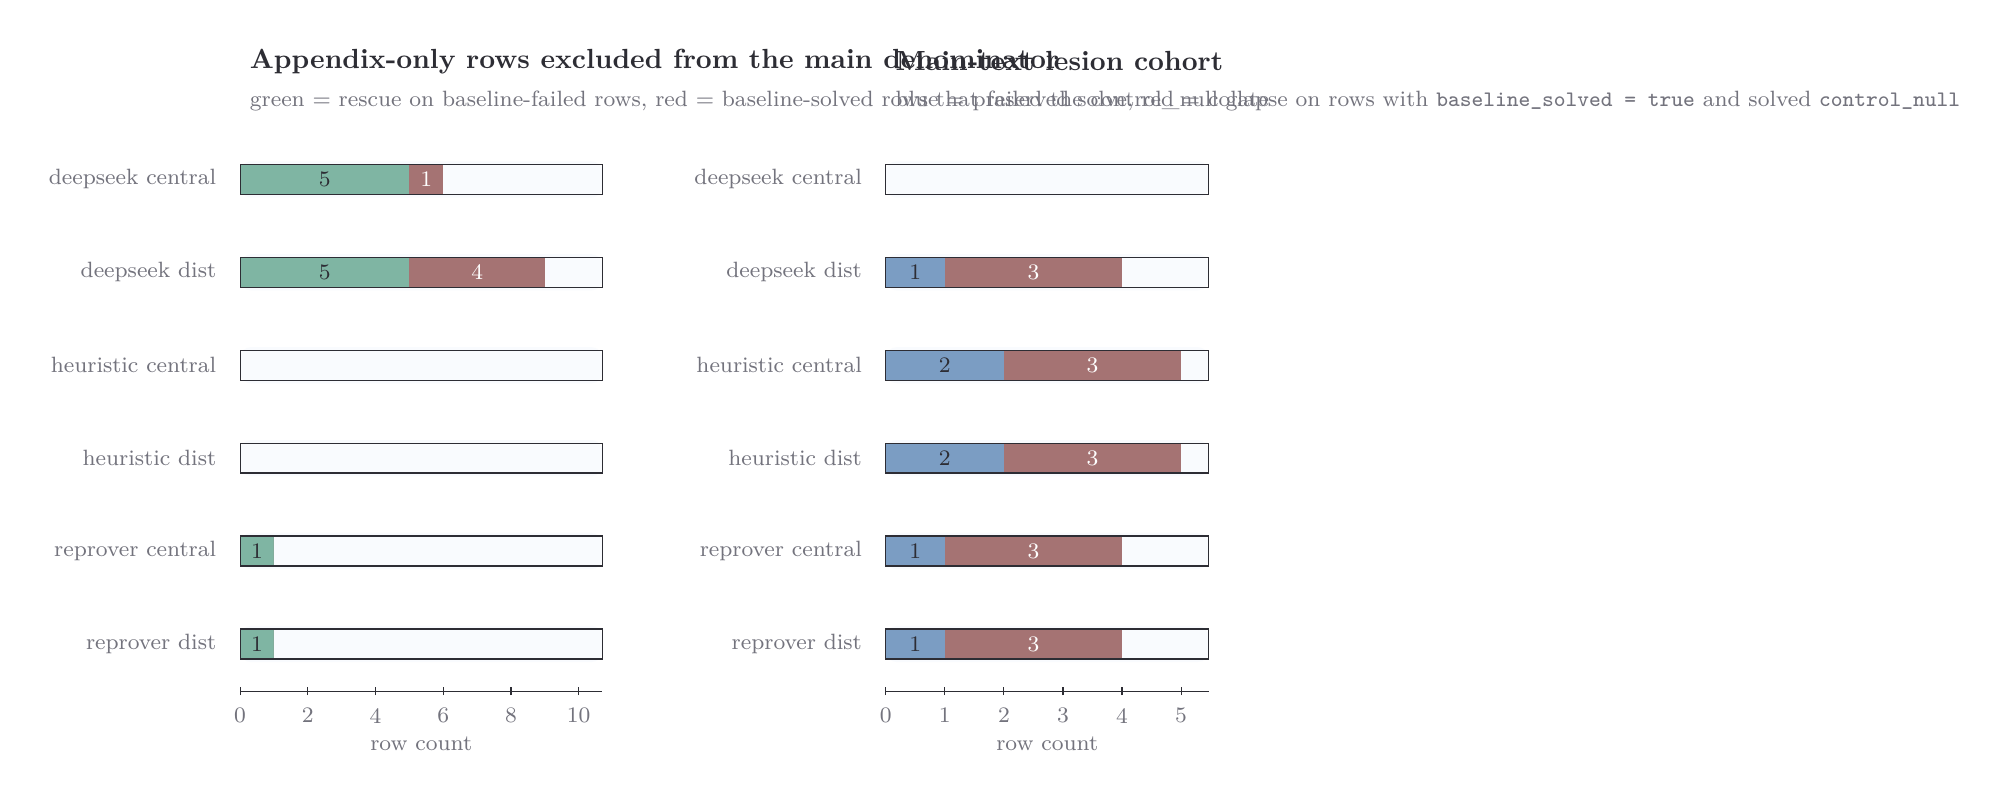
\begin{tikzpicture}[
    every node/.style={font=\small},
    show background rectangle,
    background rectangle/.style={fill=white}
]

\def\rowgap{1.18}
\def\leftunit{0.43}
\def\rightunit{0.75}

\node[paneltitle, anchor=west] at (0, 6.65) {Appendix-only rows excluded from the main denominator};
\node[annot, anchor=west] at (0, 6.15) {green = rescue on baseline-failed rows, red = baseline-solved rows that failed the control\_null gate};

\foreach \i/\label/\rescue/\unstable in {
    0/{deepseek central}/5/1,
    1/{deepseek dist}/5/4,
    2/{heuristic central}/0/0,
    3/{heuristic dist}/0/0,
    4/{reprover central}/1/0,
    5/{reprover dist}/1/0
} {
    \pgfmathsetmacro{\y}{5.15 - \i * \rowgap}
    \pgfmathsetmacro{\rescueend}{\rescue * \leftunit}
    \pgfmathsetmacro{\stackend}{(\rescue + \unstable) * \leftunit}
    \node[annot, anchor=east] at (-0.18, \y) {\label};
    \path[fill=basin1!18, rounded corners=4pt] (0, \y - 0.23) rectangle (4.6, \y + 0.23);
    \fill[accentgreen!75] (0, \y - 0.19) rectangle (\rescueend, \y + 0.19);
    \fill[blocked!78] (\rescueend, \y - 0.19) rectangle (\stackend, \y + 0.19);
    \draw[ink, line width=0.45pt] (0, \y - 0.19) rectangle (4.6, \y + 0.19);
    \ifnum\rescue>0
        \node[annot, text=ink] at (0.5 * \rescueend, \y) {\rescue};
    \fi
    \ifnum\unstable>0
        \pgfmathsetmacro{\unstablecenter}{(\rescue + 0.5 * \unstable) * \leftunit}
        \node[annot, text=white] at (\unstablecenter, \y) {\unstable};
    \fi
}

\draw[ink, line width=0.5pt] (0, -1.35) -- (4.6, -1.35);
\foreach \x/\label in {0/0, 0.86/2, 1.72/4, 2.58/6, 3.44/8, 4.30/10} {
    \draw[ink, line width=0.4pt] (\x, -1.40) -- (\x, -1.30);
    \node[annot, anchor=north] at (\x, -1.44) {\label};
}
\node[annot] at (2.3, -2.02) {row count};

\begin{scope}[shift={(8.2, 0)}]
    \node[paneltitle, anchor=west] at (0, 6.65) {Main-text lesion cohort};
    \node[annot, anchor=west] at (0, 6.15) {blue = preserved solve, red = collapse on rows with \texttt{baseline\_solved = true} and solved \texttt{control\_null}};

    \foreach \i/\label/\pres/\coll in {
        0/{deepseek central}/0/0,
        1/{deepseek dist}/1/3,
        2/{heuristic central}/2/3,
        3/{heuristic dist}/2/3,
        4/{reprover central}/1/3,
        5/{reprover dist}/1/3
    } {
        \pgfmathsetmacro{\y}{5.15 - \i * \rowgap}
        \pgfmathsetmacro{\presend}{\pres * \rightunit}
        \pgfmathsetmacro{\stackend}{(\pres + \coll) * \rightunit}
        \node[annot, anchor=east] at (-0.18, \y) {\label};
        \path[fill=basin1!18, rounded corners=4pt] (0, \y - 0.23) rectangle (4.1, \y + 0.23);
        \fill[accentblue!78] (0, \y - 0.19) rectangle (\presend, \y + 0.19);
        \fill[blocked!78] (\presend, \y - 0.19) rectangle (\stackend, \y + 0.19);
        \draw[ink, line width=0.45pt] (0, \y - 0.19) rectangle (4.1, \y + 0.19);
        \ifnum\pres>0
            \node[annot, text=ink] at (0.5 * \presend, \y) {\pres};
        \fi
        \ifnum\coll>0
            \pgfmathsetmacro{\collcenter}{(\pres + 0.5 * \coll) * \rightunit}
            \node[annot, text=white] at (\collcenter, \y) {\coll};
        \fi
    }

    \draw[ink, line width=0.5pt] (0, -1.35) -- (4.1, -1.35);
    \foreach \x/\label in {0/0, 0.75/1, 1.50/2, 2.25/3, 3.00/4, 3.75/5} {
        \draw[ink, line width=0.4pt] (\x, -1.40) -- (\x, -1.30);
        \node[annot, anchor=north] at (\x, -1.44) {\label};
    }
    \node[annot] at (2.05, -2.02) {row count};
\end{scope}

\end{tikzpicture}
\end{document}
